\graphicspath{{./chapters/01-design/figures/}}

\chapter{Design}
\label{chap:design}

The DLXY is a processor architecture based on the DLX architecture described
in \textit{Fundamentals of Computer Design - Patterson, Hennessy}, with few
modifications.

\bigskip
DLXY main characteristics include:
\begin{itemize}
	\item Instruction set: RISC (partial DLX instruction set support)
	\item Memory addressing modes: dedicated Load \& Store instructions only
	\item Data types and parallelism: integer, 32 bits
	\item Endianness: bi-endian
	\item Datapath: in-order 5 stages pipeline
	\item Control unit: hardwired
\end{itemize}

\section{Outside}

\subsection{Interface}
The DLXY core is designed to be inserted in an environment which provides:
\begin{itemize}
	\item the \textbf{clock signal}
	\item some \textbf{configuration signals}
	\item the \textbf{instruction memory}
	\item the \textbf{data memory}
\end{itemize}

\begin{figure}[H]
	\centering
	\frame{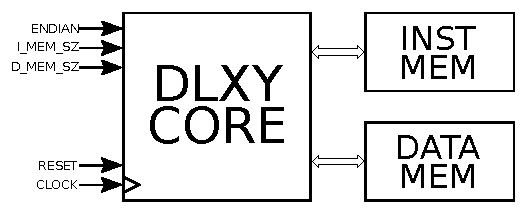
\includegraphics[width=.5\textwidth]{top_mounted}}
	\caption{The DLXY core inserted in the appropriate environment.}
	\label{fig:env_top}
\end{figure}

\subsubsection{Configuration signals}
When the \textbf{reset signal} is:
\begin{itemize}
	\item inactive (low): the processor runs in the \textit{operating mode}:
		the execution flows according to the content of the instruction
		memory
	\item active (high): the processor runs in the \textit{configuration mode}:
		\begin{itemize}
			\item internal status is cleared and is set up for
				starting the execution from address 0 of the
				instruction memory
			\item values of the configuration signals are stored
				and will be used during the operating mode
		\end{itemize}
\end{itemize}

\begin{table}[H]
	\centering
	\begin{tabular}{ll}
		\hline
		\rowcolor{gray!50}
		Signal & Meaning \\
		\texttt{ENDIAN} & \texttt{'0'}: big endian; \texttt{'1'}: little endian \\
		\rowcolor{gray!25}
		\texttt{I\_MEM\_SZ} & Size (in lines) of the physical instruction
			memory (max $2^{32}$) \\
		\texttt{D\_MEM\_SZ} & Size (in lines) of the physical data memory 
			(max $2^{32}$) \\
		\hline
	\end{tabular}
	\label{tab:config_signals}
\end{table}

\subsubsection{Memories}
Both instruction and data memory must support \textbf{asynchronous reading} and
the \textbf{delay} of the response must be below \textbf{one clock cycle}.

The \textbf{data memory} must also provide \textbf{synchronous writing} capabilities.

\bigskip
Table \ref{tab:i_mem_specs} and \ref{tab:d_mem_specs} show the required memory
specifications in detail.

\begin{table}[H]
	\centering
	\begin{tabular}{llll}
		\hline
		\rowcolor{gray!50}
		Access type & Data size & Address & Timing \\
		Read & Word & Word aligned & Asynchronous \\
		\hline
	\end{tabular}
	\caption{Instruction memory specifications.}
	\label{tab:i_mem_specs}
\end{table}

\begin{table}[H]
	\centering
	\begin{tabular}{lllll}
		\hline
		\rowcolor{gray!50}
		Access type & Data size & Address & Timing & Control signal \\
		Read & Word & Word aligned & Asynchronous & \texttt{RD = "11"} \\
		\rowcolor{gray!25}
		Read & Half word & Half word aligned & Asynchronous & \texttt{RD = "10"} \\
		Read & Byte & Any & Asynchronous & \texttt{RD = "01"} \\
		\rowcolor{gray!25}
		Write & Word & Word aligned & Synchronous & \texttt{WR = "11"} \\
		Write & Half word & Half word aligned & Synchronous & \texttt{WR = "10"} \\
		\rowcolor{gray!25}
		Write & Byte & Any & Synchronous & \texttt{WR = "01"} \\
		\hline
	\end{tabular}
	\caption{Data memory specifications.}
	\label{tab:d_mem_specs}
\end{table}

\subsection{Instruction set}
The DLXY instruction set is a \textbf{subset of the original DLX} one:
it supports all the \textbf{instructions involving integers} (except for
\texttt{LHI}, which can be easily obtained using other instructions).

A modified version of \texttt{MULT} instruction between signed half words is
supported too.

\bigskip
There are \textbf{32 general purpose integer 32-bits registers} (\texttt{R0-R31})
which can be used as sources or destination of instructions.

\texttt{R0} has a special behavior: when it is used as source it always
\textbf{evaluates to 0} and when it is used as destination the writeback
has no effect.

\bigskip
Figure \ref{fig:encoding} shows the encoding of each instruction type, while
tables \ref{tab:r_type_inst}, \ref{tab:i_type_inst} and \ref{tab:j_type_inst}
display all the supported instructions.

\begin{figure}[H]
	\centering
	\frame{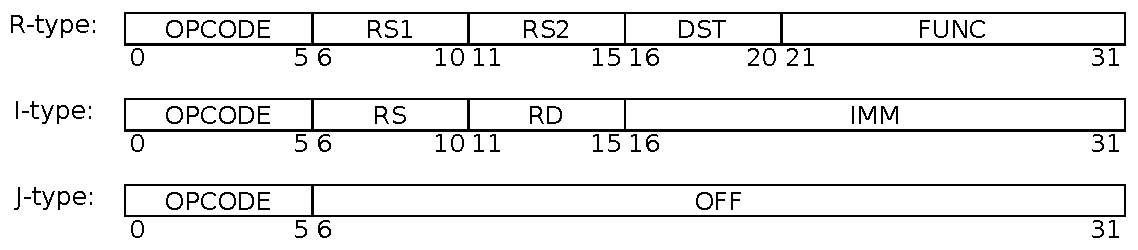
\includegraphics[width=.75\textwidth]{encoding}}
	\caption{The DLXY instruction encoding.}
	\label{fig:encoding}
\end{figure}

\begin{table}[H]
	\centering
	\begin{tabular}{ll}
		\hline
		\rowcolor{gray!50}
		Symbol & Result \\
		\texttt{SLL} & \texttt{RF(RD) <= RF(RS1) logic shifted to the left by unsigned(RF(RS2)) bits} \\
		\rowcolor{gray!25}
		\texttt{SRL} & \texttt{RF(RD) <= RF(RS1) logic shifted to the right by unsigned(RF(RS2)) bits} \\
		\texttt{SRA} & \texttt{RF(RD) <= RF(RS1) arithmetic shifted to the right by unsigned(RF(RS2)) bits} \\
		\rowcolor{gray!25}
		\texttt{ADD} & \texttt{RF(RD) <= signed(RF(RS1)) + signed(RF(RS2))} \\
		\texttt{ADDU} & \texttt{RF(RD) <= unsigned(RF(RS1)) + unsigned(RF(RS2))} \\
		\rowcolor{gray!25}
		\texttt{SUB} & \texttt{RF(RD) <= signed(RF(RS1)) - signed(RF(RS2))} \\
		\texttt{SUBU} & \texttt{RF(RD) <= unsigned(RF(RS1)) - unsigned(RF(RS2))} \\
		\rowcolor{gray!25}
		\texttt{MULT} & \texttt{RF(RD) <= signed(low\_half(RF(RS1))) * signed(low\_half(RF(RS2)))} \\
		\texttt{AND} & \texttt{RF(RD) <= RF(RS1) AND RF(RS2)} \\
		\rowcolor{gray!25}
		\texttt{OR} & \texttt{RF(RD) <= RF(RS1) OR RF(RS2)} \\
		\texttt{XOR} & \texttt{RF(RD) <= RF(RS1) XOR RF(RS2)} \\
		\rowcolor{gray!25}
		\texttt{SEQ} & \texttt{RF(RD) <= 1 when (RF(RS1) = RF(RS2)) else 0} \\
		\texttt{SNE} & \texttt{RF(RD) <= 1 when (RF(RS1) != RF(RS2)) else 0} \\
		\rowcolor{gray!25}
		\texttt{SLT} & \texttt{RF(RD) <= 1 when (signed(RF(RS1)) < signed(RF(RS2))) else 0} \\
		\texttt{SGT} & \texttt{RF(RD) <= 1 when (signed(RF(RS1)) > signed(RF(RS2))) else 0} \\
		\rowcolor{gray!25}
		\texttt{SLE} & \texttt{RF(RD) <= 1 when (signed(RF(RS1)) <= signed(RF(RS2))) else 0} \\
		\texttt{SGE} & \texttt{RF(RD) <= 1 when (signed(RF(RS1)) >= signed(RF(RS2))) else 0} \\
		\rowcolor{gray!25}
		\texttt{SLTU} & \texttt{RF(RD) <= 1 when (unsigned(RF(RS1)) < unsigned(RF(RS2))) else 0} \\
		\texttt{SGTU} & \texttt{RF(RD) <= 1 when (unsigned(RF(RS1)) > unsigned(RF(RS2))) else 0} \\
		\rowcolor{gray!25}
		\texttt{SLEU} & \texttt{RF(RD) <= 1 when (unsigned(RF(RS1)) <= unsigned(RF(RS2))) else 0} \\
		\texttt{SGEU} & \texttt{RF(RD) <= 1 when (unsigned(RF(RS1)) >= unsigned(RF(RS2))) else 0} \\
		\hline
	\end{tabular}
	\caption{R-type instructions supported by DLXY.}
	\label{tab:r_type_inst}
\end{table}

\begin{table}[H]
	\centering
	\begin{tabular}{ll}
		\hline
		\rowcolor{gray!50}
		Symbol & Result \\
		\texttt{BEQZ} & \texttt{PC <= (PC + 4 + signed(IMM)) when (RF(RS) = 0) else (PC + 4)} \\
		\rowcolor{gray!25}
		\texttt{BNEZ} & \texttt{PC <= (PC + 4 + signed(IMM)) when (RF(RS) != 0) else (PC + 4)} \\
		\texttt{ADDI} & \texttt{RF(RD) <= signed(RF(RS)) + signed(IMM)} \\
		\rowcolor{gray!25}
		\texttt{ADDUI} & \texttt{RF(RD) <= unsigned(RF(RS)) + unsigned(IMM)} \\
		\texttt{SUBI} & \texttt{RF(RD) <= signed(RF(RS)) - signed(IMM)} \\
		\rowcolor{gray!25}
		\texttt{SUBUI} & \texttt{RF(RD) <= unsigned(RF(RS)) - unsigned(IMM)} \\
		\texttt{ANDI} & \texttt{RF(RD) <= RF(RS) AND unsigned(IMM)} \\
		\rowcolor{gray!25}
		\texttt{ORI} & \texttt{RF(RD) <= RF(RS) OR unsigned(IMM)} \\
		\texttt{XORI} & \texttt{RF(RD) <= RF(RS) XOR unsigned(IMM)} \\
		\rowcolor{gray!25}
		\texttt{SLLI} & \texttt{RF(RD) <= RF(RS) logic shifted to the left by unsigned(IMM) bits} \\
		\texttt{SRLI} & \texttt{RF(RD) <= RF(RS) logic shifted to the right by unsigned(IMM) bits} \\
		\rowcolor{gray!25}
		\texttt{SRAI} & \texttt{RF(RD) <= RF(RS) arithmetic shifted to the right by unsigned(IMM) bits} \\
		\texttt{SEQI} & \texttt{RF(RD) <= 1 when (RF(RS) = signed(IMM)) else 0} \\
		\rowcolor{gray!25}
		\texttt{SNEI} & \texttt{RF(RD) <= 1 when (RF(RS) != signed(IMM)) else 0} \\
		\texttt{SLTI} & \texttt{RF(RD) <= 1 when (signed(RF(RS)) < signed(IMM)) else 0} \\
		\rowcolor{gray!25}
		\texttt{SGTI} & \texttt{RF(RD) <= 1 when (signed(RF(RS)) > signed(IMM)) else 0} \\
		\texttt{SLEI} & \texttt{RF(RD) <= 1 when (signed(RF(RS)) <= signed(IMM)) else 0} \\
		\rowcolor{gray!25}
		\texttt{SGEI} & \texttt{RF(RD) <= 1 when (signed(RF(RS)) >= signed(IMM)) else 0} \\
		\texttt{SLTUI} & \texttt{RF(RD) <= 1 when (unsigned(RF(RS)) < unsigned(IMM)) else 0} \\
		\rowcolor{gray!25}
		\texttt{SGTUI} & \texttt{RF(RD) <= 1 when (unsigned(RF(RS)) > unsigned(IMM)) else 0} \\
		\texttt{SLEUI} & \texttt{RF(RD) <= 1 when (unsigned(RF(RS)) <= unsigned(IMM)) else 0} \\
		\rowcolor{gray!25}
		\texttt{SGEUI} & \texttt{RF(RD) <= 1 when (unsigned(RF(RS)) >= unsigned(IMM)) else 0} \\
		\texttt{LB} & \texttt{RF(RD) <= signed(low\_byte(MEM(RF(RS) + signed(IMM))))} \\
		\rowcolor{gray!25}
		\texttt{LH} & \texttt{RF(RD) <= signed(low\_half(MEM(RF(RS) + signed(IMM))))} \\
		\texttt{LW} & \texttt{RF(RD) <= MEM(RF(RS) + signed(IMM))} \\
		\rowcolor{gray!25}
		\texttt{LBU} & \texttt{RF(RD) <= unsigned(low\_byte(MEM(RF(RS) + signed(IMM))))} \\
		\texttt{LHU} & \texttt{RF(RD) <= unsigned(low\_half(MEM(RF(RS) + signed(IMM))))} \\
		\rowcolor{gray!25}
		\texttt{SB} & \texttt{MEM(RF(RS) + signed(IMM)) <= low\_byte(RF(RD))} \\
		\texttt{SH} & \texttt{MEM(RF(RS) + signed(IMM)) <= low\_half(RF(RD))} \\
		\rowcolor{gray!25}
		\texttt{SW} & \texttt{MEM(RF(RS) + signed(IMM)) <= RF(RD)} \\
		\texttt{NOP} & Null \\
		\hline
	\end{tabular}
	\caption{I-type instructions supported by DLXY.}
	\label{tab:i_type_inst}
\end{table}

\begin{table}[H]
	\centering
	\begin{tabular}{ll}
		\hline
		\rowcolor{gray!50}
		Symbol & Result \\
		\texttt{J} & \texttt{PC <= PC + 4 + signed(OFF)} \\
		\rowcolor{gray!25}
		\texttt{JAL} & \texttt{PC <= PC + 4 + signed(OFF); RF(R31) <= PC + 4} \\
		\texttt{JR} & \texttt{PC <= RF(low\_5\_bits(OFF))} \\
		\rowcolor{gray!25}
		\texttt{JALR} & \texttt{PC <= RF(low\_5\_bits(OFF)); RF(R31) <= PC + 4} \\
		\hline
	\end{tabular}
	\caption{J-type instructions supported by DLXY.}
	\label{tab:j_type_inst}
\end{table}

\subsubsection{Assembler}
The code to be loaded to the instruction memory can be easily generated using
the assembler located in \texttt{assembly/assembler}.
In \texttt{assembly/code} there are also some example programs.

\section{Architecture}
The DLXY core is made up of two components: an hardwired \textbf{control unit}
and a pipelined \textbf{datapath}.

\begin{figure}[H]
	\centering
	\frame{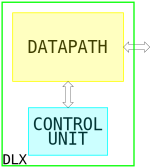
\includegraphics[width=.35\textwidth]{architecture}}
	\caption{The DLXY architecture.}
	\label{fig:architecture}
\end{figure}

\subsection{Datapath}
The DLXY datapath is a customized DLX pipeline, which still maintains the
\textbf{in-order 5 stages} structure but includes some other features such as
data forwarding, anticipated branch target computation, disabling out-of-bound
memory accesses, configurable endianness.

\bigskip
The pipeline stages are:
\begin{enumerate}
	\item \textbf{Fetch stage} (IF):
		\begin{itemize}
			\item select program counter according to previous branch
				taken status
			\item read instruction memory at address corresponding
				to program counter and forward the read data to
				the next stage
			\item perform conversion of the read data from big to
				little endian, if the processor is configured in
				big endian
			\item compute next sequential program counter
		\end{itemize}
	\item \textbf{Decode stage} (ID):
		\begin{itemize}
			\item forward data from following stages, if necessary
			\item extract data from encoded instruction
			\item extend immediate operands
			\item read from registerfile
			\item compute branch target
			\item compare sources with 0 and with destination of
				other instructions in the pipeline
		\end{itemize}
	\item \textbf{Execute stage} (EX):
		\begin{itemize}
			\item forward data from following stages, if necessary
			\item execute the selected operation
		\end{itemize}
	\item \textbf{Memory stage} (MEM):
		\begin{itemize}
			\item forward data from following stages, if necessary
			\item disable memory access if address exceeds data
				memory size
			\item align address according to access size
			\item read/write data memory
			\item perform conversion of the read/written data from
				little to big endian, if the processor is
				configured in big endian
		\end{itemize}
	\item \textbf{Writeback stage} (WB):
		\begin{itemize}
			\item write instruction result to register file
		\end{itemize}
\end{enumerate}

At the \textbf{steady state} (when no hazard happens) all the 5 stages operates
in parallel on different data, completing one instruction per clock cycle, as
shown in figure \ref{fig:pipeline_steady}.
\begin{figure}[H]
	\centering
	\frame{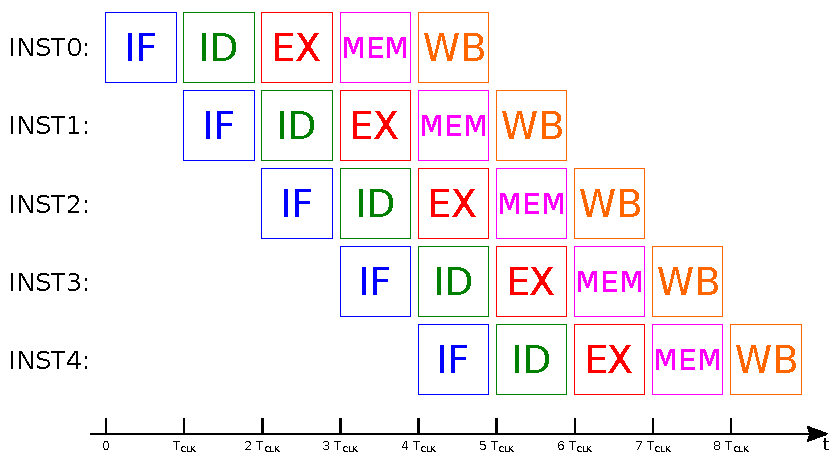
\includegraphics[width=.75\textwidth]{pipeline_steady}}
	\caption{The DLXY pipeline at the steady state.}
	\label{fig:pipeline_steady}
\end{figure}

\subsection{Control unit}
The DLXY control unit operates in the \textbf{decode stage} of each instruction
and is in charge of the generation of control signals which depend on:
\begin{itemize}
	\item \underline{instruction code} $\Rightarrow$ \textbf{instruction decoding}
	\item \underline{other instructions} in the pipeline $\Rightarrow$
		\textbf{hazard management}
\end{itemize}

\subsubsection{Hazard management}

\paragraph{Control hazards} \mbox{} \\
At the steady state the fetch unit automatically updates the program counter
with the address of the next sequential instruction.
When the instruction in execution is a \textbf{taken branch} this automatic
mechanism leads to the fetch of a wrong instruction: this is a
\textbf{control hazard}.

\bigskip
In order to solve control hazards, the control unit \textbf{converts
the instruction following a taken branch into a \texttt{NOP}} (disabling any
possible write, both to the register file and to the data memory, and disabling
any possible taken branch), since that instruction shouldn't have been fetched,
and informs the fetch unit to \textbf{use the target value} computed in the
decode stage as next program counter. This solution introduces therefore a
\textbf{penalty of one clock cycle} for each taken branch.

\bigskip
If a conditional branch is not taken the execution can proceed without any
penalty to pay: this technique is called \textbf{static untaken branch prediction}.

\begin{figure}[H]
	\centering
	\frame{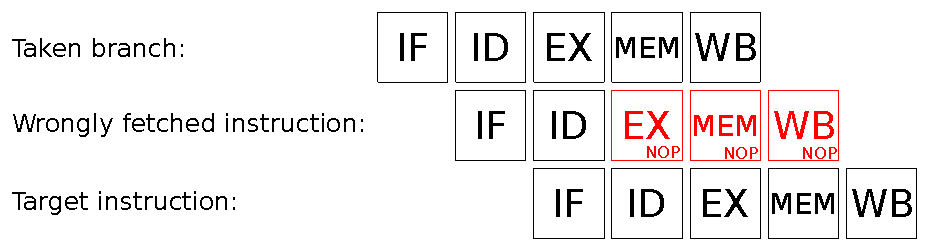
\includegraphics[width=.75\textwidth]{ctrl_hazard}}
	\caption{The DLXY pipeline when a control hazard occurs.}
	\label{fig:ctrl_hazard}
\end{figure}

\paragraph{Data hazards} \mbox{} \\
In an in-order pipeline the only possible data hazard is the \textbf{Read After
Write} hazard, which occurs when an instruction $I_B$ source operand matches
another instruction $I_A$ destination operand and $I_B$ enters the pipeline
before $I_A$ exits it.

\bigskip
The DLXY solves these hazards forwarding data or inserting stalls, depending on
$I_A$ and $I_B$ instruction types and their relative position in the pipeline.

\bigskip
A \textbf{stall} consists in disabling:
\begin{itemize}
	\item writes to both register file and data memory
	\item branches
	\item load to registers between decode and fetch units
\end{itemize}

\bigskip
The \textbf{producer result types} are:
\begin{enumerate}
	\item \textbf{ALU}: it is produced by the ALU, therefore it will be
		ready after the EX stage
	\item \textbf{LOAD}: it is loaded from the data memory, therefore it
		will be ready after the MEM stage
	\item \textbf{NULL}: it does not affect the registerfile, therefore it
		cannot cause any data hazard
\end{enumerate}

\bigskip
The \textbf{consumer operand types} are:
\begin{enumerate}
	\item \textbf{ID}: it is needed in the ID stage
	\item \textbf{EX}: it is needed in the EX stage
	\item \textbf{MEM}: it is needed in the MEM stage
\end{enumerate}

\bigskip
Table \ref{tab:data_hazard} displays the data hazard management in detail.

\begin{table}[H]
	\centering
	\begin{tabular}{cccc}
		\hline
		\rowcolor{gray!50}
		Producer result type & Producer instruction stage &
			Consumer operand type & Hazard solution \\
		ALU &	EX &	ID &	Stall \\
		\rowcolor{gray!25}
		ALU &	MEM &	ID &	Forward \\
		ALU &	WB &	ID &	Forward \\
		\hdashline
		\rowcolor{gray!25}
		ALU & 	EX &	EX &	Forward \\
		ALU & 	MEM &	EX &	Forward \\
		\rowcolor{gray!25}
		ALU & 	WB &	EX &	Forward \\
		\hdashline
		ALU & 	EX &	MEM &	Forward \\
		\rowcolor{gray!25}
		ALU & 	MEM &	MEM &	Forward \\
		ALU & 	WB &	MEM &	Forward \\
		\hdashline
		\rowcolor{gray!25}
		LOAD & 	EX &	ID &	Stall \\
		LOAD & 	MEM &	ID &	Stall \\
		\rowcolor{gray!25}
		LOAD & 	WB &	ID &	Forward \\
		\hdashline
		LOAD & 	EX &	EX &	Stall \\
		\rowcolor{gray!25}
		LOAD & 	MEM &	EX &	Forward \\
		LOAD & 	WB &	EX &	Forward \\
		\hdashline
		\rowcolor{gray!25}
		LOAD & 	EX &	MEM &	Forward \\
		LOAD & 	MEM &	MEM &	Forward \\
		\rowcolor{gray!25}
		LOAD & 	WB &	MEM &	Forward \\
		\hline
	\end{tabular}
	\caption{Data hazard management (producer instruction stage is where
		$I_A$ is located when $I_B$ is in ID stage)}
	\label{tab:data_hazard}
\end{table}

\section{Implementation}
The DLXY has been implemented in \texttt{VHDL}; most of the code is written in a
\textbf{behavioral} style: this makes it more future proof for two main reasons:
\begin{itemize}
	\item better \textbf{maintainability}: since behavioral code is much
		more readable, it is easier for the designer to find possible
		bugs and modifying existing code
	\item bigger \textbf{design space} for synthesis tools: the behavioral
		code specifies what the ciruit should do and the tool decides
		how this should be done and it is free to apply any optimization:
		advancement in the tools technology can be reflected in better
		optimized circuit
\end{itemize}

\subsection{Datapath}
The DLXY datapath is made up of \textbf{one unit for each pipeline stage}.
Between each stage and the previous one there are some \textbf{pipeline registers},
which contain both control and data signals and are loaded with new values every
clock cycle.

There is also a group of registers between the decode and the fetch units, which
can be disabled in case of data hazards.

\bigskip
Figure \ref{fig:datapath} shows an overview of the datapath internals.

\begin{figure}[H]
	\centering
	\frame{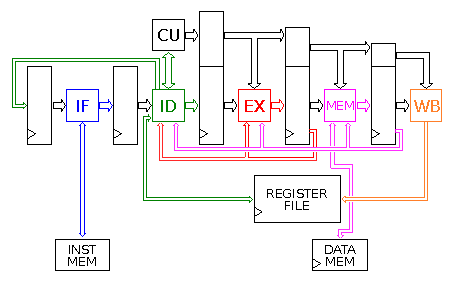
\includegraphics[width=.75\textwidth]{datapath}}
	\caption{The DLXY datapath.}
	\label{fig:datapath}
\end{figure}

\bigskip
The following subsections show a possible implementation for each datapath unit
(the synthesizer might produce slightly different circuits, with the same
functionality, depending on optimizations it applies).

\bigskip
In the schematics there are some common blocks, such as:
\begin{itemize}
	\item \textbf{Multiplexers}:
		\begin{itemize}
			\item \underline{Input(s):} 2 or more data signals,
				1 selection signal
			\item \underline{Output(s):} selected data signal
		\end{itemize}
	\item \textbf{Adders}:
		\begin{itemize}
			\item \underline{Input(s):} 2 signed/unsigned data signals
			\item \underline{Output(s):} sum between the inputs
		\end{itemize}
	\item \textbf{Comparators}:
		\begin{itemize}
			\item \underline{Input(s):} 2 unsigned data signals
			\item \underline{Output(s):} result of comparison
				(equality, inequality, magnitude) between the
				inputs
		\end{itemize}
	\item \textbf{Extenders}:
		\begin{itemize}
			\item \underline{Input(s):} 1 data signal
			\item \underline{Output(s):} data signal extended on
				a bigger number of bits, adding to the MSBs:
				'0's, if it is a zero extender or a value equal
				to the original MSB, if it is a sign extender
		\end{itemize}
\end{itemize}

\subsubsection{Fetch unit}
\begin{figure}[H]
	\centering
	\frame{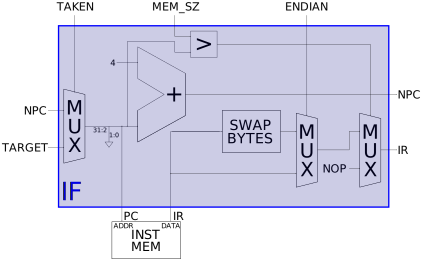
\includegraphics[width=.75\textwidth]{fetch_unit}}
	\caption{The DLXY fetch unit.}
	\label{fig:fetch_unit}
\end{figure}
\subsubsection{Decode unit}
\begin{figure}[H]
	\centering
	\frame{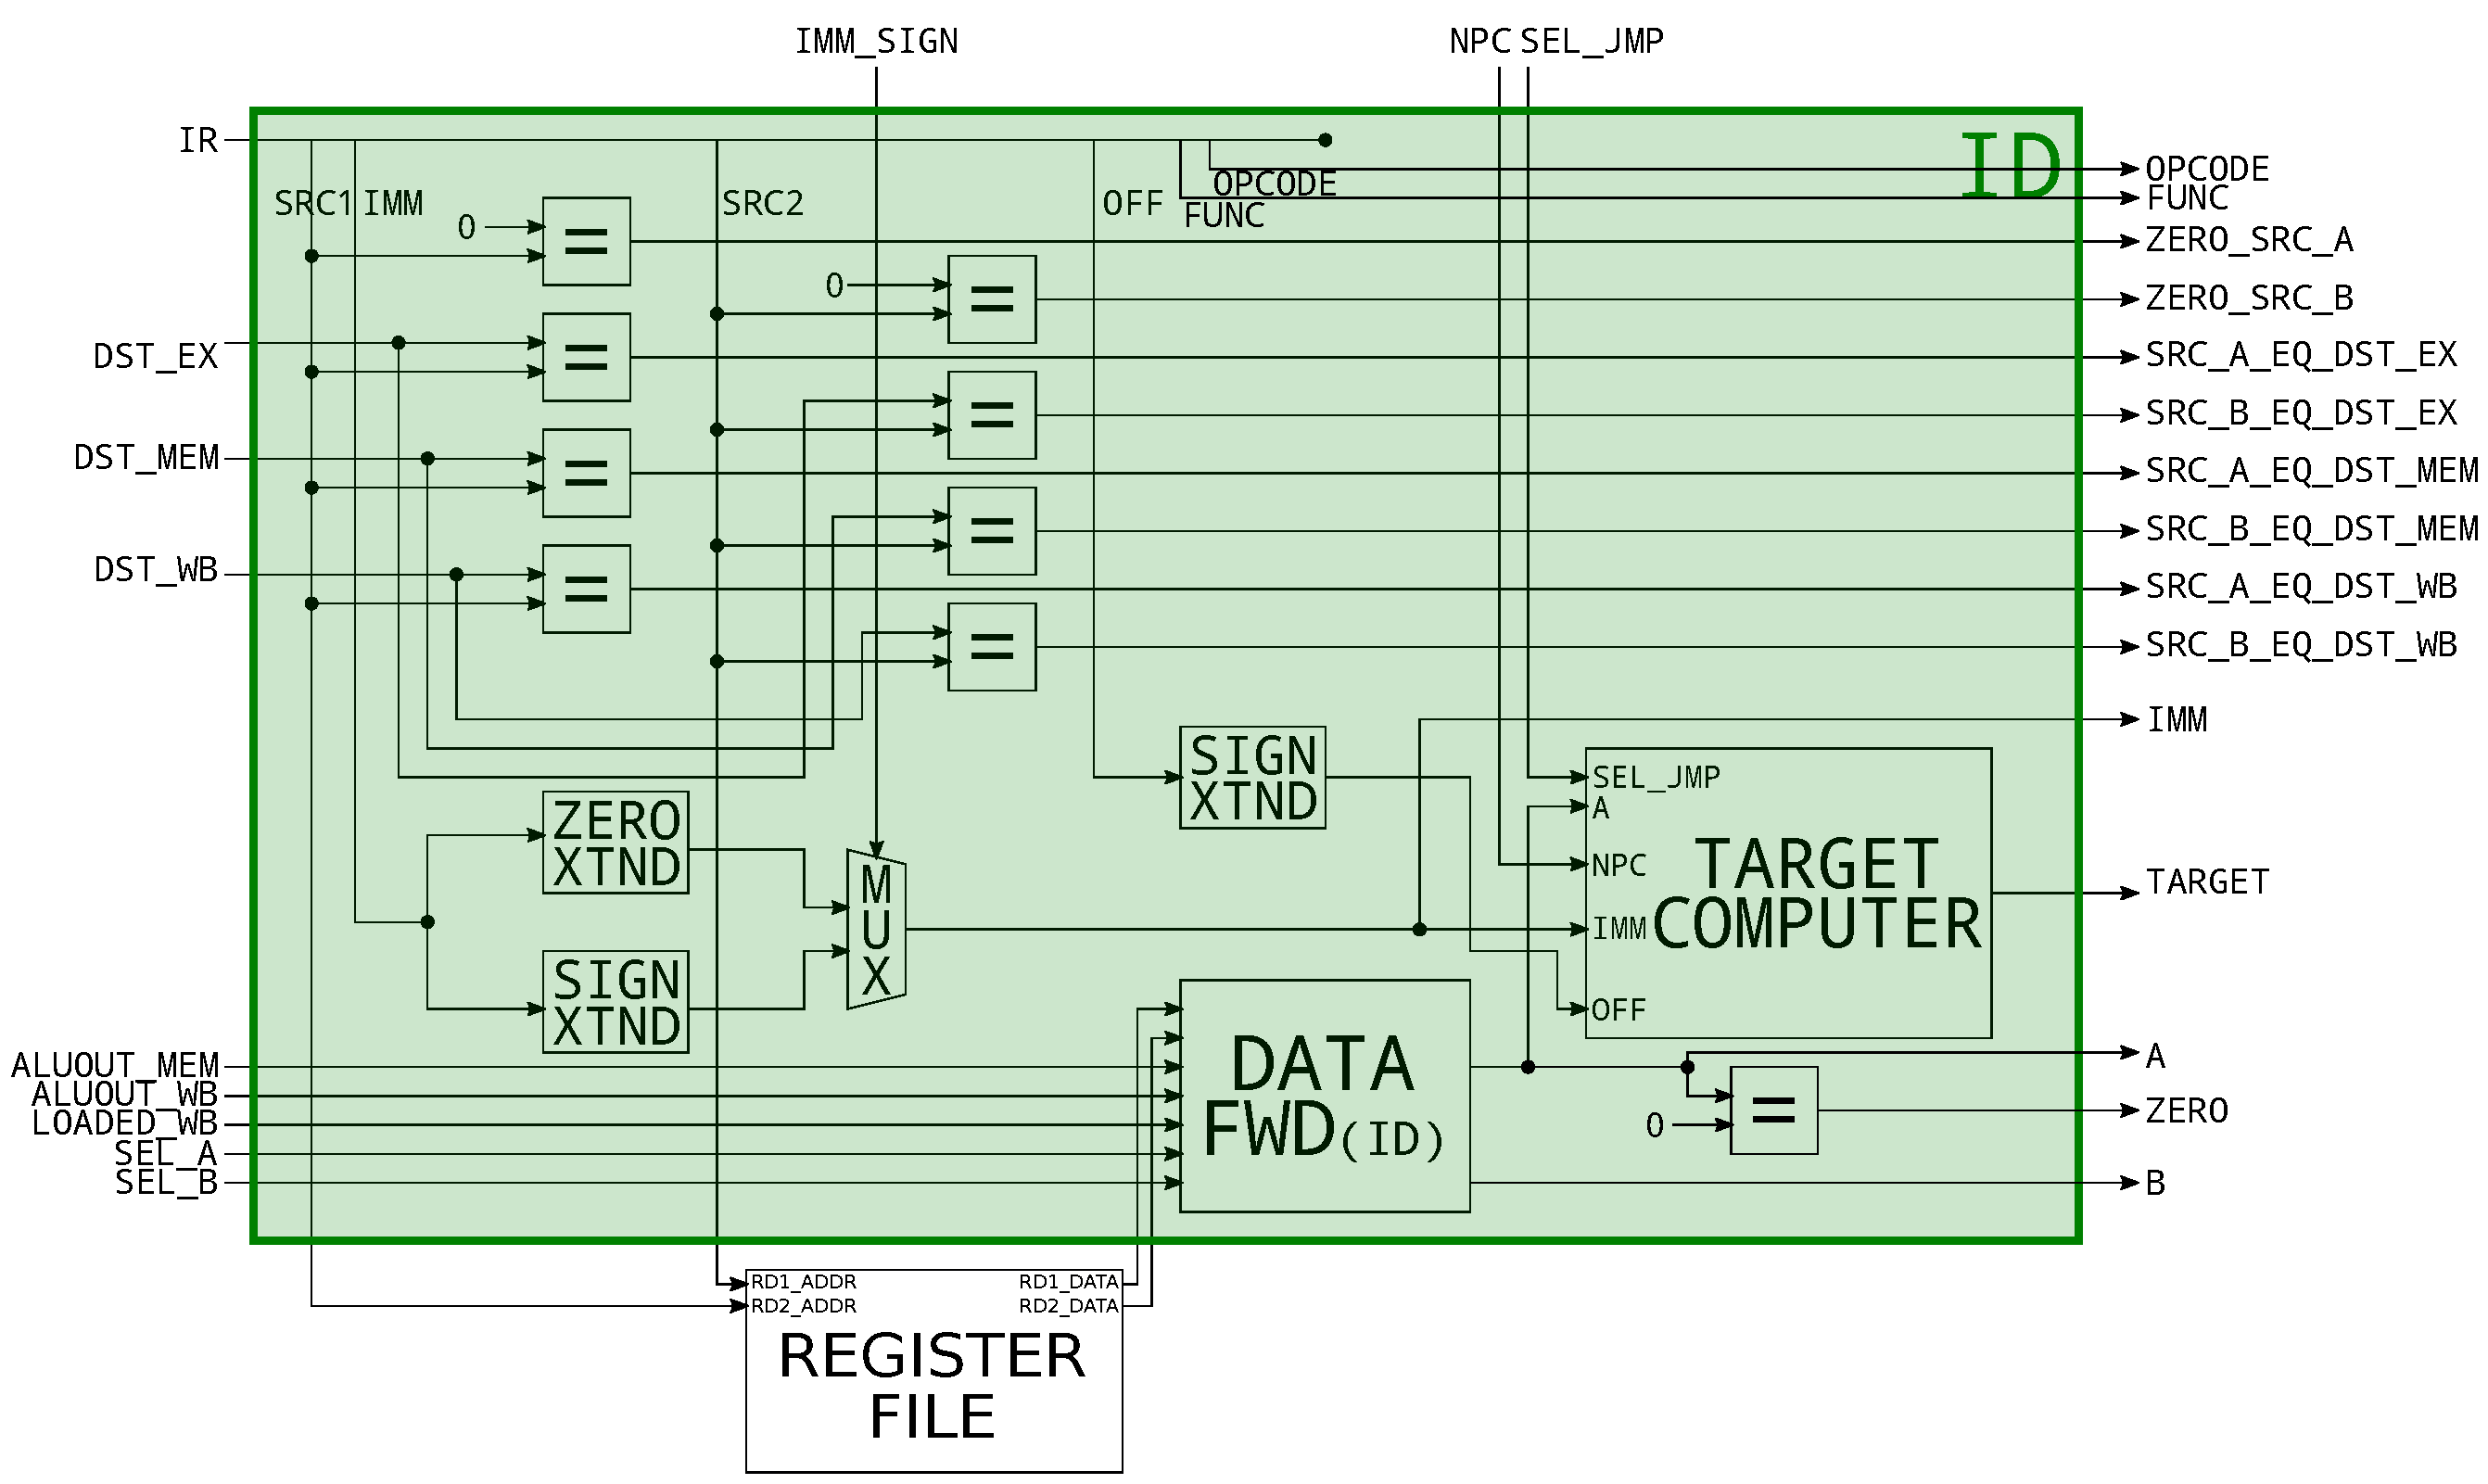
\includegraphics[width=\textwidth]{decode_unit}}
	\caption{The DLXY decode unit.}
	\label{fig:decode_unit}
\end{figure}
\paragraph{Data forwarder (ID)} \mbox{} \\
\begin{figure}[H]
	\centering
	\frame{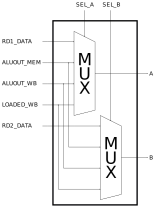
\includegraphics[width=.3\textwidth]{id_fwd}}
	\caption{The DLXY decode unit data forwarder.}
	\label{fig:id_fwd}
\end{figure}
\paragraph{Target computer} \mbox{} \\
\begin{figure}[H]
	\centering
	\frame{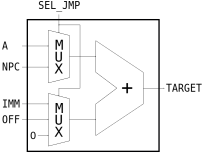
\includegraphics[width=.5\textwidth]{target_computer}}
	\caption{The DLXY decode unit target computer.}
	\label{fig:target_computer}
\end{figure}
\paragraph{Register file} \mbox{} \\
The DLXY register file provides \textbf{2 asynchronous read ports} and
\textbf{1 synchronous write port}.

\bigskip
Since it is inserted in one of the most critical stages of the pipeline, it must
be simple and fast: no additional feature has been included.

In particular, a \textit{windowed register file} has been discarded not only for
the additional hardware complexity requirement, but also because it reduces the
register space seen by the compiler: letting the compiler use the whole register
file might end up in better optimizations.
\subsubsection{Execute unit}
\begin{figure}[H]
	\centering
	\frame{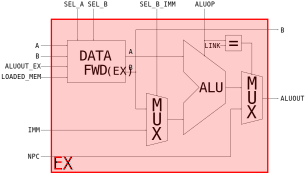
\includegraphics[width=.7\textwidth]{execute_unit}}
	\caption{The DLXY execute unit.}
	\label{fig:execute_unit}
\end{figure}

\paragraph{ALU} \mbox{} \\
The DLXY ALU supports all the operations required by the instruction set.
Some components have been described making use of standard libraries, while
other have been explicitly described.

Among the explicitly described components there are:
\begin{itemize}
	\item \textbf{Adder}: \\
		it is a performance-oriented adder based on the \texttt{Pentium 4}
		adder: it is composed of a sparse tree \textbf{carry lookahead}
		generator and a carry select \textbf{sum generator}.
		Both operands and result are on 32 bits.

		Differently from the original structure, the DLXY adder accepts
		a \textbf{carry in}, in order to support the subtraction
		(since \texttt{-A = NOT (A) + 1}, if the second operand is
		bitwise negated and the carry in is set to \texttt{'1'}, the adder
		performs a subtraction).

		Another difference from the \texttt{P4} adder is that DLXY one
		outputs an \textbf{overflow} signal, which is set to \texttt{'1'}
		whenever a signed overflow occurs.
	\item \textbf{Comparator}: \\
		in order to limit the occupied area, it reuses the adder,
		configured as subtractor: according to the subtraction result,
		the carry out and the overflow flag, it performs any magnitude
		comparison, both signed and unsigned.
	\item \textbf{Multiplier}: \\
		it is an implementation of the Booth algorithm.
		Its operands are on 16 bits and its result is on 32 bits: thanks
		to this sizing, no overflow is possible.
\end{itemize}

\subsubsection{Memory unit}
\begin{figure}[H]
	\centering
	\frame{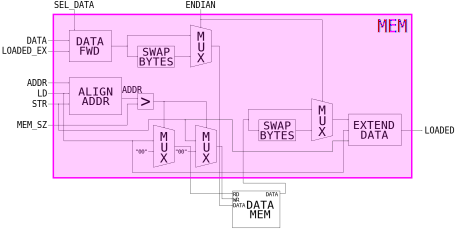
\includegraphics[width=\textwidth]{memory_unit}}
	\caption{The DLXY memory unit.}
	\label{fig:memory_unit}
\end{figure}

\paragraph{Align address} \mbox{} \\
\begin{itemize}
	\item \underline{Inputs}:
		\begin{itemize}
			\item \texttt{ADDRESS}: 32 bits signal
			\item \texttt{LD}: 2 bits signal:

				\texttt{"00"} = no load; \texttt{"01"} = load byte;
				\texttt{"10"} = load half word; \texttt{"11"} = load word
			\item \texttt{STR}: 2 bits signal

				\texttt{"00"} = no store; \texttt{"01"} = store byte;
				\texttt{"10"} = store half word; \texttt{"11"} = store word
		\end{itemize}
	\item \underline{Outputs}:
		\begin{itemize}
			\item \texttt{ADDRESS}:
				\begin{itemize}
					\item when load or store a word: word aligned (2 LSBs to \texttt{0})
					\item when load or store an half word: half word aligned (LSB to \texttt{0})
					\item otherwise: untouched
				\end{itemize}
		\end{itemize}
\end{itemize}

\subsubsection{Write unit}
\begin{figure}[H]
	\centering
	\frame{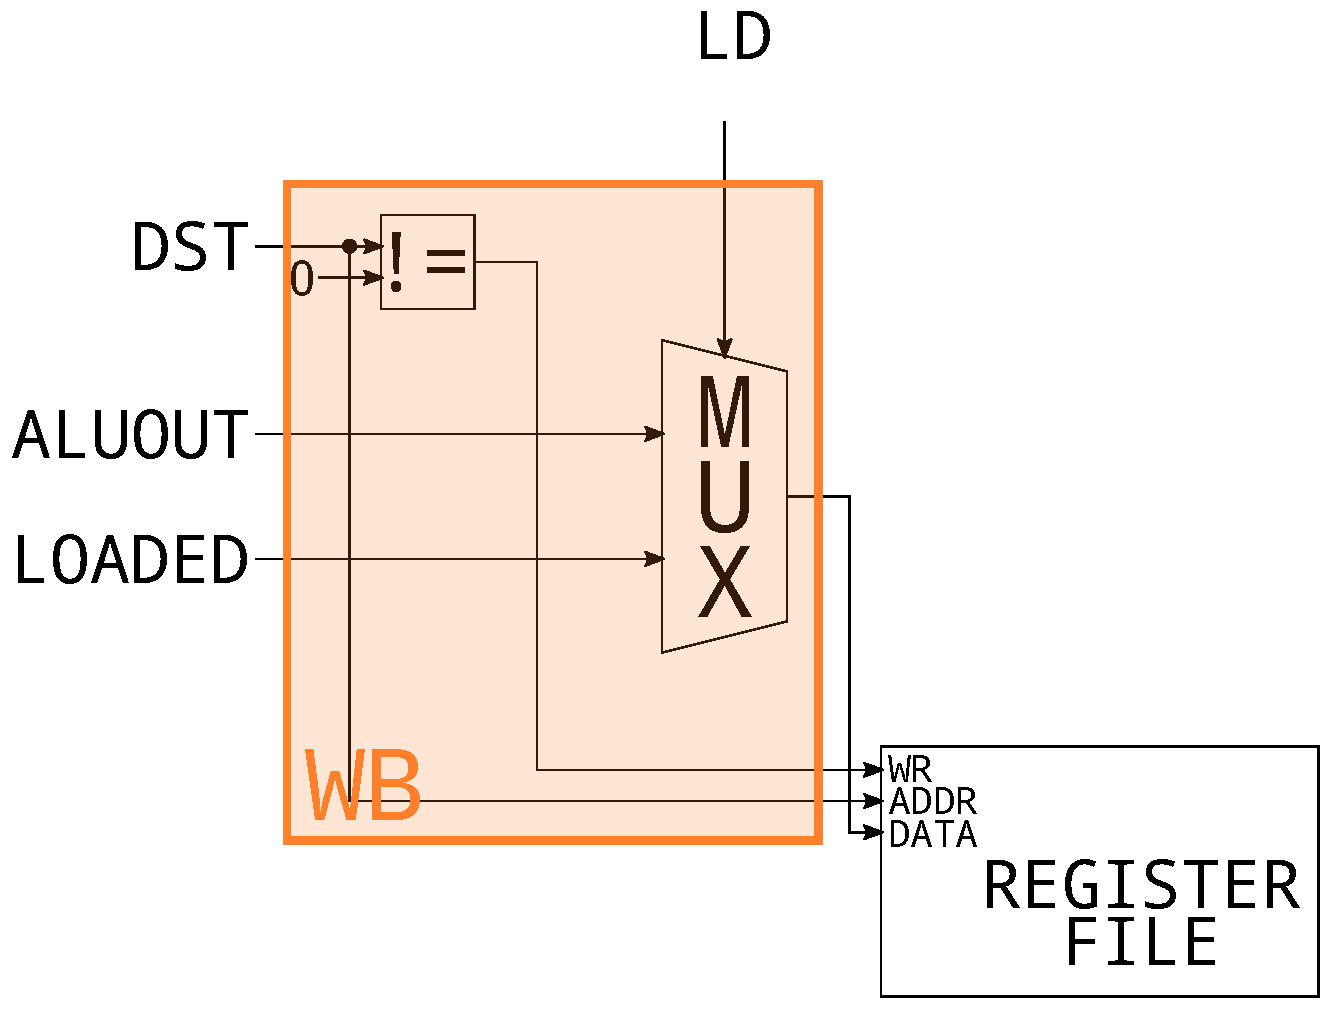
\includegraphics[width=.5\textwidth]{write_unit}}
	\caption{The DLXY write unit.}
	\label{fig:write_unit}
\end{figure}

\subsubsection{Forwarding subsystem}
The forwarding subsystem is distributed in ID, EX and MEM stages.

If it is not possible to forward a certain data to a certain stage, the control
unit would insert a stall, until it is possible to ensure that all data is
up-to-date when it is used.

Figures \ref{fig:fwd_a} and \ref{fig:fwd_b} show the forwarding subsystem alone,
extracted from the datapath (the forwarding of A operand ends in EX stage since
there is no instruction requiring its value in MEM stage).
\begin{figure}[H]
	\centering
	\frame{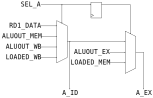
\includegraphics[width=.5\textwidth]{fwd_a}}
	\caption{The DLXY forwarding subsystem for A operand.}
	\label{fig:fwd_a}
\end{figure}
\begin{figure}[H]
	\centering
	\frame{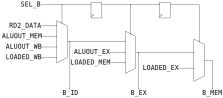
\includegraphics[width=.8\textwidth]{fwd_b}}
	\caption{The DLXY forwarding subsystem for B operand.}
	\label{fig:fwd_b}
\end{figure}

\subsection{Control unit}
\subsubsection{Design style considerations}
The DLXY control unit is made up of different components (as shown in figure
\ref{fig:control_unit}):
\begin{itemize}
	\item \textbf{Configuration register}: asynchronous memory which stores
		the processor configuration
	\item \textbf{Instruction decoder}: combinational circuit which translates
		the code of the instruction in the decode stage into control signals
	\item \textbf{Data forwarder}: combinational circuit which generates the
		signals controlling the forwarding subsystem
	\item \textbf{Stall generator}: combinational circuit which introduces
		stalls in the pipeline, when it is necessary for ensuring
		correct results
\end{itemize}

It is worth noting that the control unit generates all the control signals
needed by any instruction, in every pipeline stage: the \textbf{correct timing}
of these signals is then ensured by the \textbf{pipeline registers}.

\bigskip
The implementation style follows the \textbf{hardwired} principles: it is an
ad-hoc combinational circuit (except for the configuration register), therefore
it is possible to get \underline{better performance} and \underline{lower power}
consumption (with respect to other styles, such as microprogrammed control units)
at the expense of \underline{lower maintainability}.

\bigskip
Since the DLXY is quite a simple core, the hardwired design style had been the
natural choice.

\begin{figure}[H]
	\centering
	\frame{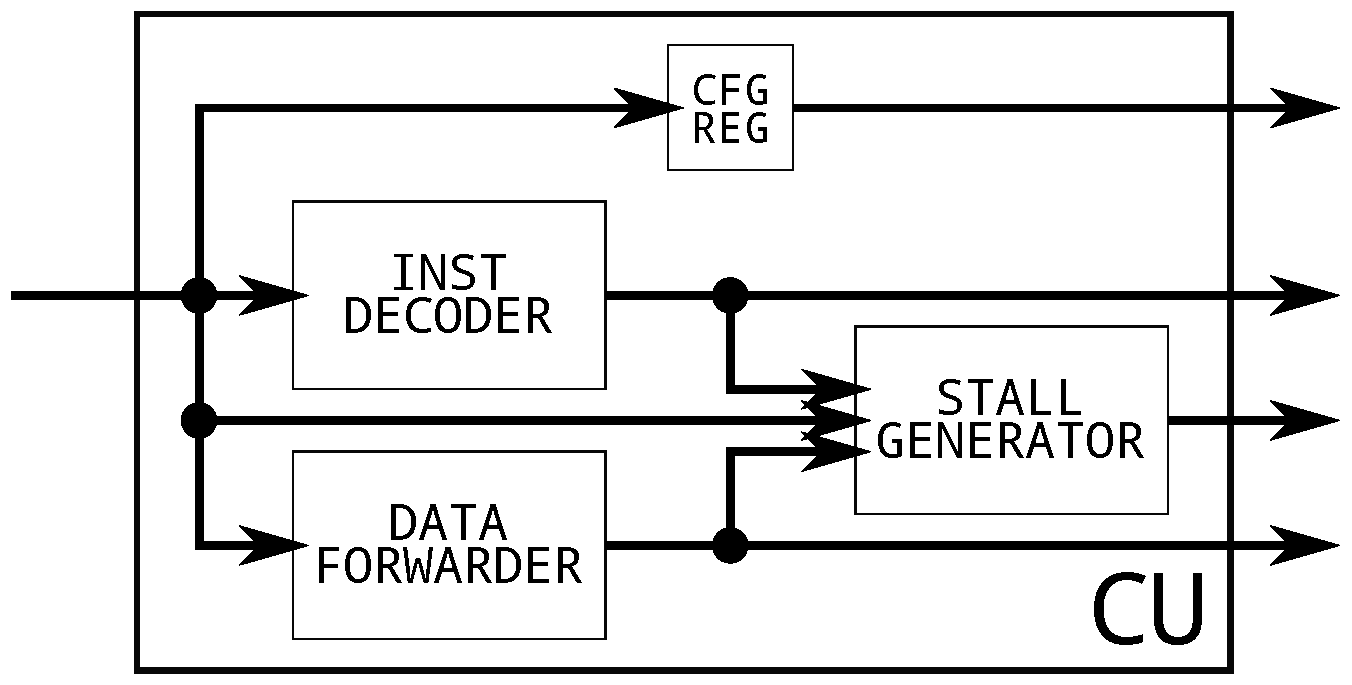
\includegraphics[width=.7\textwidth]{control_unit}}
	\caption{The DLXY control unit.}
	\label{fig:control_unit}
\end{figure}

